% !TEX program = pdflatex
% NOTE: IEEEtran 版本建议使用 pdfLaTeX 编译。
\documentclass[journal]{IEEEtran}
\usepackage{cite}
\usepackage{amsmath}
\usepackage{amssymb}
\usepackage{graphicx}
\IfFileExists{orcidlink.sty}{\usepackage{orcidlink}}{\providecommand{\orcidlink}[1]{}}
\usepackage{tikz-cd}
\usetikzlibrary{arrows.meta,positioning}

\title{Physics-Guided Learned Compensation of Structured Mismatch in Reduced-Reference Cylindrical Aperture 3-D mmW Imaging}
%\title{ReMiC-Net: A Reference-Surface-Aware Mismatch Compensation Network for Reduced-Reference Cylindrical Aperture 3-D Imaging}
\author{Yun Su\orcidlink{0009-0008-5831-9344}, Weixian Tan\orcidlink{0000-0001-9071-9470} \IEEEmembership{Member, IEEE}, Yifan Dong\orcidlink{0000-0002-3155-6437}, Wei Xu\orcidlink{0000-0002-8045-8817} \IEEEmembership{Member, IEEE}, Pingping Huang\orcidlink{0000-0001-7720-1183} \IEEEmembership{Member, IEEE}
}

\begin{document}
\maketitle

\begin{abstract}
Near-field cylindrical aperture radar imaging is an important technique for high-resolution three-dimensional reconstruction in security screening, nondestructive testing, and short-range sensing. However, accurate cylindrical aperture reconstruction requires spatially varying spherical-wave compensation, while fast reference-surface-based algorithms may introduce structured approximation mismatch when the number of reference cylindrical surfaces is aggressively reduced. In this paper, we propose a physics-guided learned compensation framework for reduced-reference cylindrical aperture 3-D imaging. The proposed method retains a reduced-reference cylindrical imaging operator as a low-complexity physical backbone and introduces ReMiC-Net, a reference-surface-aware mismatch compensation network for residual correction and structural restoration. Instead of directly regressing the final image, ReMiC-Net learns the residual between the coarse reduced-reference reconstruction and the target reflectivity, while explicitly using reference-surface-aware geometric metadata, including shell assignment, nearest-reference deviation, valid field-of-view mask, and support prior. A dual-branch architecture with FiLM-style modulation is adopted to inject geometry-aware conditioning into volumetric feature extraction. In addition, an auxiliary support prediction head is introduced to improve extended-target structural preservation. Simulated and experimental results demonstrate that the proposed method substantially improves reconstruction quality, support continuity, and speed--quality trade-off while maintaining a runtime close to the reduced-reference physical backbone. The proposed framework provides an efficient and interpretable learning-assisted solution for compensating structured model mismatch in fast cylindrical aperture 3-D imaging.
\end{abstract}

\begin{IEEEkeywords}
Cylindrical aperture imaging, millimeter-wave radar imaging, physics-guided reconstruction, reference-surface-aware learning, structured mismatch compensation.
\end{IEEEkeywords}

\section{Introduction}
Near-field millimeter-wave and microwave three-dimensional (3-D) imaging has attracted increasing attention in security screening, nondestructive testing, through-wall sensing, and biomedical inspection. Owing to the penetration capability of millimeter-wave signals through common nonmetallic materials and their nonionizing nature, active near-field radar imaging systems can provide high-resolution volumetric information of concealed or weakly visible targets. In these applications, both image quality and reconstruction speed are critical, since the imaging system is often required to reconstruct complex 3-D scenes within a limited acquisition and processing time.

Among various near-field imaging configurations, cylindrical aperture imaging is particularly attractive because it provides wide angular observation and is suitable for full-view 3-D reconstruction of human-scale or object-scale targets. However, cylindrical aperture imaging is also substantially more challenging than planar aperture imaging. Under near-field conditions, the spherical wavefront, free-space propagation loss, nonlinear range history, nonuniform wavenumber-domain sampling, and space-variant point spread function must be properly handled. As a result, the imaging operator cannot be simply represented as a global convolution, and standard fast Fourier transform (FFT)-based algorithms developed for planar apertures cannot be directly applied without additional approximations or coordinate transformations \cite{Fortuny-Guasch_Lopez-Sanchez_2001,Tan_Hong_Wang_Wu_2011,Gao_Deng_Qin_Wang_Li_2018,Wang_Yao_Song_Wang_Sun_2024}.

Backprojection (BP) and matched-filtering-based methods can accurately compensate the spherical-wave propagation path for each voxel, and are therefore commonly regarded as high-fidelity reconstruction approaches. Nevertheless, their voxel-wise coherent summation leads to high computational cost, which restricts their use in real-time 3-D imaging. To improve efficiency, a variety of frequency-domain and wavenumber-domain algorithms have been developed for near-field cylindrical and MIMO imaging. For example, nonplanar measurements can be backpropagated to a planar aperture before applying 3-D range migration \cite{Fortuny-Guasch_Lopez-Sanchez_2001}; spherical wave decomposition, circular convolution, and nonuniform FFT can be exploited for efficient MIMO cylindrical holographic imaging \cite{Gao_Deng_Qin_Wang_Li_2018}; and mixed-domain formulations have been proposed to address space-variant spectral characteristics in more complicated near-field MIMO-SAR configurations \cite{Wang_Yao_Song_Wang_Sun_2024}. These methods have significantly advanced fast 3-D near-field imaging, but they still rely on carefully designed analytical approximations and often exhibit a trade-off between computational efficiency and reconstruction fidelity.

Another important class of fast cylindrical aperture imaging methods is based on reference cylindrical surfaces. The basic idea is to divide the imaging region into cylindrical surfaces with different radii and construct matched filters with respect to selected reference surfaces. By reusing the matched-filtering functions associated with these reference surfaces, the repeated computation of spatially varying focusing kernels can be reduced. Tan et al. developed a spherical-wave 3-D imaging algorithm for cylindrical scanning geometries that explicitly considers wavefront curvature and free-space propagation loss \cite{Tan_Hong_Wang_Wu_2011}. More recently, a high-precision millimeter-wave cylindrical aperture holographic imaging algorithm was proposed, where the imaging region is divided into cylindrical surfaces of different radii, reference cylindrical surfaces are selected according to imaging accuracy and phase-error control, and the complexity of repeated matched-filter computation is reduced \cite{Tan}. This reference-surface strategy provides an efficient and physically interpretable backbone for cylindrical aperture imaging.

Despite its efficiency, reference-surface-based imaging naturally introduces approximation errors when the number of reference surfaces is aggressively reduced. A dense reference-surface library improves focusing accuracy but increases computational cost, whereas a reduced-reference implementation is fast but no longer perfectly matched to the true radial position of every voxel. The resulting error is not random noise; it is a structured, geometry-dependent mismatch governed by the assigned reference surface, radial deviation from that surface, angular observation geometry, and valid field-of-view support. This structured mismatch becomes particularly harmful for extended targets, where boundary continuity, support integrity, and thin structures are more important than isolated peak localization.

Deep learning provides a promising way to compensate such model-induced reconstruction errors. Recent studies in computational electromagnetic imaging have shown that purely data-driven networks may suffer from limited interpretability and generalization, while physics-embedded learning can combine analytical imaging operators with trainable neural networks to improve both efficiency and reconstruction quality \cite{Guo_Huang_Li_Zhang_Eldar_2023}. In near-field 3-D radar imaging, Manisali et al. proposed a two-stage physics-based learned reconstruction framework, where an adjoint physical operator first maps radar measurements to the image domain and a 3-D U-Net then refines the intermediate reconstruction for extended targets \cite{Manisali_Oral_Oktem_2024}. This demonstrates the effectiveness of using a physics-based warm start followed by a deep volumetric network. Related learning-based 3-D SAR and millimeter-wave imaging methods, such as RMIST-Net, further show that embedding analytical operators into neural reconstruction can improve computational efficiency \cite{Wang_Wei_Liang_Zeng_Wang_Shi_Zhang_2022}. However, most existing learning-based radar imaging methods focus on sparse reconstruction, compressive sensing, MIMO array configurations, or generic image-domain refinement. They do not explicitly address the structured mismatch induced by reduced-reference cylindrical aperture imaging.

Model mismatch has also been recognized as a key issue in learning-based 3-D radar reconstruction. For instance, MAda-Net shows that a fixed observation model cannot accurately represent spatially varying observation models in TomoSAR, and that such model inconsistency can cause nonnegligible imaging errors that cannot be fully eliminated by network parameter optimization alone \cite{Wang_Liu_Zhu_Liu_Ding_Zeng_2023}. This observation is closely related to reduced-reference cylindrical imaging: using a small number of reference surfaces is equivalent to forcing a spatially varying cylindrical imaging process to be represented by a limited set of approximate reference models. Therefore, the network should not be treated as a generic post-processing module. Instead, it should be explicitly informed of the reference-surface assignment and the local severity of the approximation error.

In addition, extended-target reconstruction requires more than voxel-wise intensity correction. Recent studies in deep-learning-based TomoSAR reconstruction have shown that spatial features such as edges, regular shapes, and structural continuity can provide useful constraints for 3-D reconstruction, especially when the target scene contains prominent spatial structures \cite{Zeng_Zhan_Ren_Ma_Liu_Shi_Wei_Wang_Zhang_2025}. For reduced-reference cylindrical aperture imaging, extended targets are also the most challenging cases, because reference-surface mismatch may lead to support fragmentation, boundary deformation, and shape distortion. Therefore, a structure-aware compensation strategy is needed to recover not only the intensity distribution but also the target support.

Motivated by these observations, this paper proposes a physics-guided learned compensation framework for structured mismatch in reduced-reference cylindrical aperture 3-D imaging. The proposed method, termed \emph{ReMiC-Net}, is a Reference-Surface-Aware Mismatch Compensation Network for Reduced-Reference Cylindrical Aperture 3-D Imaging. Instead of replacing the analytical imaging operator, ReMiC-Net retains a reduced-reference cylindrical aperture imaging operator as a fast physical backbone. The coarse reconstruction obtained from this backbone is then refined by a residual compensation network conditioned on reference-surface-aware geometric metadata, including shell assignment, nearest-reference deviation, valid field-of-view mask, and support prior. In addition, an auxiliary support prediction head is introduced to improve extended-target structural preservation, including support continuity, boundary integrity, and thin-structure recovery.

The main contributions of this paper are summarized as follows.

\begin{itemize}
    \item We formulate the approximation error of reduced-reference cylindrical aperture imaging as a structured, geometry-dependent mismatch rather than generic image degradation. This formulation provides a problem-driven perspective for learning-assisted fast cylindrical aperture 3-D imaging.

    \item We propose ReMiC-Net, a reference-surface-aware residual compensation network that explicitly uses reference-surface metadata to guide mismatch correction. The network is designed to compensate the reduced-reference approximation error while preserving the low-complexity advantage of the physical backbone.

    \item We design a reference-surface-aware geometry conditioning strategy to guide residual mismatch compensation. The network explicitly uses shell assignment, nearest-reference deviation, valid field-of-view information, and support prior, allowing the compensation behavior to adapt to the local severity of reduced-reference approximation error.

    \item We incorporate an auxiliary support prediction task to improve extended-target structure preservation. The support supervision encourages the network to recover continuous target regions, thin structures, and boundaries that are easily distorted by reduced-reference approximation.

    \item We conduct systematic simulations and experimental evaluations, including point-target validation, extended-target reconstruction, ablation studies, support-structure analysis, runtime comparison, robustness tests, and measured-data validation. The results demonstrate that the proposed method can significantly improve reconstruction quality while maintaining a runtime close to the reduced-reference physical backbone.
\end{itemize}

The remainder of this paper is organized as follows. Section~II introduces the mathematical background of cylindrical aperture 3-D imaging and reduced-reference approximation. Section~III presents the proposed ReMiC-Net framework, including the reference-surface-aware input representation, network architecture, residual compensation strategy, and support-aware loss design. Section~IV reports simulated and experimental results. Section~V concludes this paper and discusses future work.

\section{Mathematical Background}
\label{sec:math_background}

This section formulates the cylindrical aperture near-field imaging model and clarifies the source of the structured mismatch considered in this work. The exact reference-surface selections used for \emph{ref3}, \emph{ref5}, \emph{ref7}, and \emph{ref9} are reported in the experimental section, while this section focuses on the general forward model and the reduced-reference approximation mechanism.

\subsection{Cylindrical Aperture Imaging Geometry}
\label{subsec:geometry}

Consider a monostatic cylindrical aperture imaging system, where a transmit/receive antenna samples the scattered field on a cylindrical surface. The antenna position is denoted as
\begin{equation}
\mathbf{r}'(\phi',z')=
\left[\rho_0\cos\phi',\ \rho_0\sin\phi',\ z'\right]^T,
\label{eq:antenna_position}
\end{equation}
where \(\rho_0\) is the radius of the cylindrical scan, \(\phi'\) is the azimuth sampling angle, and \(z'\) is the elevation position. A voxel in the imaging domain is represented in cylindrical coordinates as
\begin{equation}
\mathbf{r}(\rho,\phi,z)=
\left[\rho\cos\phi,\ \rho\sin\phi,\ z\right]^T,
\label{eq:voxel_position}
\end{equation}
where \(\rho\), \(\phi\), and \(z\) denote the radial, azimuthal, and elevation coordinates, respectively. The propagation distance between the antenna and the voxel is then
\begin{equation}
R(\rho,\phi,z;\phi',z')=
\sqrt{\rho_0^2+\rho^2-2\rho_0\rho\cos(\phi-\phi')+(z-z')^2}.
\label{eq:range}
\end{equation}
This spherical-wave distance term is the central geometric quantity in cylindrical aperture near-field imaging. It makes the phase history dependent on the voxel position and prevents the cylindrical case from being reduced to a simple space-invariant Cartesian convolution.

Fig.~\ref{fig:cylindrical_geometry} shows a schematic illustration of the cylindrical scanning geometry and the use of multiple reference cylindrical surfaces. The concrete reference radii used in the comparative baselines are listed later in Section~IV.

\begin{figure}[!t]
\centering
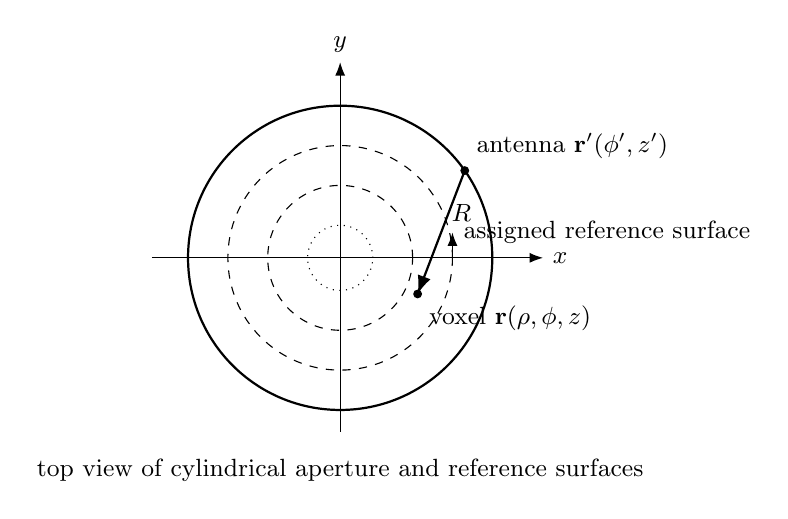
\begin{tikzpicture}[scale=0.92, >=Latex]
    % coordinate axes
    \draw[->] (-2.6,0) -- (2.8,0) node[right] {\small $x$};
    \draw[->] (0,-2.4) -- (0,2.7) node[above] {\small $y$};

    % reference surfaces top view
    \draw[thick] (0,0) circle (2.1);
    \draw[dashed] (0,0) circle (1.55);
    \draw[dashed] (0,0) circle (1.00);
    \draw[dotted] (0,0) circle (0.45);

    % antenna position
    \coordinate (ant) at ({2.1*cos(35)},{2.1*sin(35)});
    \filldraw[black] (ant) circle (1.5pt);
    \node[above right=1pt of ant] {\small antenna $\mathbf{r}'(\phi',z')$};

    % voxel
    \coordinate (vox) at ({1.18*cos(-25)},{1.18*sin(-25)});
    \filldraw[black] (vox) circle (1.5pt);
    \node[below right=1pt of vox] {\small voxel $\mathbf{r}(\rho,\phi,z)$};

    % range arrow
    \draw[->, thick] (ant) -- (vox) node[midway, above right] {\small $R$};

    % reference label
    \draw[->] (1.55,0) -- (1.55,0.35);
    \node[right] at (1.57,0.35) {\small assigned reference surface};
    \node[below] at (0,-2.65) {\small top view of cylindrical aperture and reference surfaces};
\end{tikzpicture}
\caption{Schematic top-view illustration of cylindrical aperture imaging. The antenna samples the scattered field on a cylindrical surface, while the imaging region is represented by voxels with radial coordinate \(\rho\). Reduced-reference imaging uses only a subset of reference cylindrical surfaces to construct approximate matched filters.}
\label{fig:cylindrical_geometry}
\end{figure}

\subsection{Spherical-Wave Forward Model}
\label{subsec:forward_model}

Let \(x(\rho,\phi,z)\) denote the complex-valued 3-D reflectivity distribution of the scene. For a point scatterer, the measured response at the frequency wavenumber \(k=2\pi f/c\) can be expressed as
\begin{equation}
 y_p(k,\phi',z')=
 x(\rho,\phi,z)\frac{\exp[-j2kR(\rho,\phi,z;\phi',z')]}{R^2(\rho,\phi,z;\phi',z')},
\label{eq:point_model_full}
\end{equation}
where the exponential term represents the two-way spherical-wave phase history and \(R^{-2}\) models the free-space propagation loss. In calibrated or amplitude-compensated processing, the amplitude factor may be removed or absorbed into a weighting term, yielding the phase-dominant model
\begin{equation}
 y_p(k,\phi',z')=
 x(\rho,\phi,z)\exp[-j2kR(\rho,\phi,z;\phi',z')].
\label{eq:point_model_phase}
\end{equation}

For an extended target, the received echo is the coherent superposition of all voxel contributions:
\begin{equation}
 y(k,\phi',z')=
 \iiint_{V} x(\rho,\phi,z)
 \exp[-j2kR(\rho,\phi,z;\phi',z')]\, dV
 + n(k,\phi',z'),
\label{eq:continuous_forward}
\end{equation}
where \(V\) is the imaging volume and \(n(k,\phi',z')\) denotes measurement noise and modeling error. This model follows the linearized scattering assumption commonly adopted in holographic microwave and SAR-type imaging; multiple scattering within the object is not modeled.

After discretization, the forward model is written as
\begin{equation}
\mathbf{y}=\mathbf{A}\mathbf{x}+\mathbf{n},
\label{eq:discrete_forward}
\end{equation}
where \(\mathbf{y}\in\mathbb{C}^{M}\) is the measurement vector, \(\mathbf{x}\in\mathbb{C}^{N}\) is the discretized 3-D reflectivity vector, and \(\mathbf{A}\in\mathbb{C}^{M\times N}\) is the cylindrical near-field forward operator. The \((m,n)\)-th element of \(\mathbf{A}\) can be expressed as
\begin{equation}
 A_{m,n}=w_{m,n}\exp[-j2k_m R(\mathbf{r}_n;\phi'_m,z'_m)],
\label{eq:system_matrix}
\end{equation}
where \(w_{m,n}\) denotes the optional amplitude weighting term. When free-space propagation loss has been compensated or ignored, \(w_{m,n}=1\).

The sampling intervals along frequency, azimuth, and elevation are chosen to satisfy the cylindrical aperture sampling constraints to avoid aliasing; the detailed numerical sampling parameters used in this work are provided in Section~IV rather than repeated here.

\subsection{Matched-Filtering Reconstruction}
\label{subsec:matched_filter}

Given the cylindrical echo \(y(k,\phi',z')\), a spherical-wave matched-filtering or backprojection-type reconstruction can be written as
\begin{equation}
 \tilde{x}(\rho,\phi,z)=
 \int_{z'}\int_{\phi'}\int_{k}
 y_R(k,\phi',z')
 \exp[+j2kR(\rho,\phi,z;\phi',z')]
 k\, dk\, d\phi'\, dz',
\label{eq:matched_filter}
\end{equation}
where \(y_R(k,\phi',z')\) denotes the range-gated or amplitude-compensated echo. Eq.~\eqref{eq:matched_filter} can be interpreted as an adjoint-type operation of the forward model in Eq.~\eqref{eq:discrete_forward}. It coherently compensates the spherical-wave phase history for each candidate voxel.

However, because \(R(\rho,\phi,z;\phi',z')\) is nonlinear and spatially varying, direct evaluation of Eq.~\eqref{eq:matched_filter} over a dense 3-D grid is computationally expensive. This motivates accelerated cylindrical reconstruction methods based on wavenumber-domain processing, range stacking, or reference-surface approximation.

\subsection{Reference-Surface-Based Reconstruction}
\label{subsec:reference_surface}

Reference-surface-based cylindrical reconstruction reduces the repeated computation of spatially varying matched filters by dividing the imaging region into a sequence of cylindrical surfaces. Let the full reference-surface library be denoted by
\begin{equation}
\mathcal{S}_{\mathrm{full}}=
\{\rho_1,\rho_2,\ldots,\rho_L\}.
\label{eq:full_reference_library}
\end{equation}
For each reference radius \(\rho_l\), an approximate matched filter is constructed as
\begin{equation}
 H_l(k,\phi',z';\phi,z)=
 \exp[+j2kR(\rho_l,\phi,z;\phi',z')].
\label{eq:reference_filter}
\end{equation}
A full-reference reconstruction operator can then be abstractly represented as
\begin{equation}
 \mathbf{x}_{\mathrm{full}}=\mathcal{R}_{\mathrm{full}}(\mathbf{y}),
\label{eq:full_reconstruction}
\end{equation}
where \(\mathcal{R}_{\mathrm{full}}\) uses a sufficiently dense reference-surface library to approximate the exact spherical-wave focusing process.

In this paper, the detailed radius selections for \emph{ref3}, \emph{ref5}, \emph{ref7}, and \emph{ref9} are not listed in this background section. They are instead reported in Section~IV, together with the simulation and runtime settings, because those selections are part of the experimental protocol.

\subsection{Reduced-Reference Approximation and Structured Mismatch}
\label{subsec:structured_mismatch}

To obtain a low-complexity physical backbone, only a small subset of the full reference library is used:
\begin{equation}
\mathcal{S}_{Q}=\{\rho_{q_1},\rho_{q_2},\ldots,\rho_{q_Q}\},\quad Q\ll L.
\label{eq:reduced_library}
\end{equation}
For a voxel \(v\) with radial coordinate \(\rho(v)\), its assigned reference radius is defined as
\begin{equation}
 \rho_Q^{\ast}(v)=
 \arg\min_{\rho_q\in\mathcal{S}_{Q}} |\rho(v)-\rho_q|.
\label{eq:assigned_reference}
\end{equation}
The corresponding signed radial deviation is
\begin{equation}
 \delta\rho_Q(v)=\rho(v)-\rho_Q^{\ast}(v).
\label{eq:radial_deviation}
\end{equation}
Using this reduced library, the approximate reconstruction is denoted by
\begin{equation}
 \mathbf{x}_{Q}=\mathcal{R}_{Q}(\mathbf{y}).
\label{eq:reduced_reconstruction}
\end{equation}
In particular, the most aggressive low-complexity backbone used in this work is
\begin{equation}
 \mathbf{x}_{\mathrm{ref3}}=\mathcal{R}_{\mathrm{ref3}}(\mathbf{y}).
\label{eq:ref3_reconstruction}
\end{equation}

The reduced-reference approximation introduces a deterministic phase mismatch. For voxel \(v\) and measurement index \(m\), this mismatch can be written as
\begin{equation}
\Delta\Phi_m(v;Q)=
2k_m\left[
R(\rho(v),\phi(v),z(v);\phi'_m,z'_m)
-
R(\rho_Q^{\ast}(v),\phi(v),z(v);\phi'_m,z'_m)
\right].
\label{eq:phase_error}
\end{equation}
This phase mismatch is governed by the cylindrical geometry, the assigned reference radius, the radial deviation, the observation angle, the elevation coordinate, and the frequency. Therefore, the error induced by reduced-reference imaging is not independent random noise, but a structured, geometry-dependent approximation error.

For simulated data, the target label in this work is defined as the ground-truth reflectivity:
\begin{equation}
\mathbf{x}^{\star}=\mathbf{x}_{\mathrm{gt}}.
\label{eq:gt_label}
\end{equation}
The structured mismatch associated with the reduced-reference backbone is then defined as
\begin{equation}
 \Delta\mathbf{x}_{\mathrm{ref3}}
 =
 \mathbf{x}^{\star}-\mathbf{x}_{\mathrm{ref3}}
 =
 \mathbf{x}_{\mathrm{gt}}-\mathcal{R}_{\mathrm{ref3}}(\mathbf{y}).
\label{eq:ref3_residual}
\end{equation}
Thus, the learning problem addressed in this paper is not generic image enhancement, but compensation of the structured approximation mismatch induced by the reduced-reference cylindrical aperture operator. This motivates the ReMiC-Net framework introduced in Section~III, where the network predicts a residual correction conditioned on reference-surface-aware geometry and is further supervised by support-aware structural learning.

\section*{Notes for Integration into the Full Manuscript}
The schematic figure in Fig.~\ref{fig:cylindrical_geometry} is intentionally conceptual. In the final manuscript, it may be redrawn as a publication-quality vector figure. The concrete reference radius table for \emph{ref3}/\emph{ref5}/\emph{ref7}/\emph{ref9} should be placed in Section~IV, together with the experimental parameters.

% =========================================================
% Section III. Methodology
% File: section_III_methodology.tex
% Notes:
% 1) Replace figure file paths such as Fig2_overall_framework.pdf with your actual files.
% 2) Replace citation keys such as \cite{Tan2024,Manisali2024,Guo2023} with your BibTeX keys.
% 3) This file is designed to be included in an IEEE-style manuscript.
% =========================================================

\section{Methodology}
\label{sec:methodology}

This section presents the proposed physics-guided learned compensation framework for reduced-reference cylindrical aperture 3-D imaging. The central idea is to retain a low-complexity cylindrical physical reconstruction operator as the first-stage backbone and to learn only the structured residual mismatch induced by the reduced number of reference cylindrical surfaces. Different from a generic image-enhancement network, the proposed method is designed to be reference-surface-aware: the network is informed by cylindrical reference-surface metadata and trained to recover both reflectivity residuals and extended-target support structures.

\subsection{Cylindrical Aperture Forward Model}
\label{subsec:reduced_reference_backbone}

We consider a monostatic cylindrical near-field imaging geometry, where the transceiver samples the scattered field on a cylindrical aperture. Let a target voxel be denoted by its cylindrical coordinate $(\rho,\theta,z)$ and the transceiver position be denoted by $(\rho_0,\theta',z')$, where $\rho_0$ is the scanning radius. The propagation distance between the voxel and the transceiver is
\begin{equation}
R(\rho,\theta,z;\theta',z')=
\sqrt{\rho_0^2+\rho^2-2\rho_0\rho\cos(\theta-\theta')+(z-z')^2}.
\label{eq:distance}
\end{equation}
For a reflectivity distribution $x(\rho,\theta,z)$, the measured cylindrical echo can be written in the frequency domain as
\begin{equation}
y(k,\theta',z') = \iiint_{\mathcal{V}} x(\rho,\theta,z)
\exp[-j2kR(\rho,\theta,z;\theta',z')]\,dV + n,
\label{eq:reduced_backbone_measurement}
\end{equation}
where $k$ is the wavenumber, $\mathcal{V}$ denotes the imaging volume, and $n$ denotes measurement noise and modeling error. After discretization, the forward model is expressed as
\begin{equation}
\mathbf{y}=\mathbf{A}\mathbf{x}+\mathbf{n},
\label{eq:reduced_backbone_discrete}
\end{equation}
where $\mathbf{x}\in\mathbb{C}^{N}$ is the vectorized 3-D reflectivity volume, $\mathbf{y}\in\mathbb{C}^{M}$ is the vectorized echo measurement, and $\mathbf{A}\in\mathbb{C}^{M\times N}$ is the cylindrical forward operator. This forward model provides the physical basis for the reduced-reference reconstruction backbone. In the current magnitude-domain version of ReMiC-Net, the network does not estimate the complex reflectivity phase; therefore, complex echo-domain consistency is not imposed as a training loss.

\subsection{Reduced-Reference Cylindrical Physical Backbone}
\label{subsec:physical_backbone}

Classical cylindrical holographic imaging reconstructs the 3-D reflectivity by focusing the echo data on a sequence of reference cylindrical surfaces. A dense reference-surface library improves focusing accuracy but increases the computational burden because the matched filtering operation must be repeatedly evaluated for many radial surfaces. To obtain a low-complexity physical backbone, we use a reduced-reference cylindrical reconstruction operator.

Let the full reference-surface library be
\begin{equation}
\mathcal{P}_{\mathrm{full}}=\{0.00,0.01,0.02,\ldots,0.30\}\;\mathrm{m}.
\label{eq:backbone_reference_library}
\end{equation}
The default reduced-reference backbone uses three uniformly distributed reference surfaces:
\begin{equation}
\mathcal{P}_{\mathrm{ref3}}=\{0.00,0.15,0.30\}\;\mathrm{m}.
\label{eq:ref3_surfaces}
\end{equation}
Given the measured echo $\mathbf{y}$, the first-stage physical reconstruction is
\begin{equation}
\mathbf{x}_{\mathrm{ref3}}=\mathcal{R}_{\mathrm{ref3}}(\mathbf{y}),
\label{eq:backbone_ref3_reconstruction}
\end{equation}
where $\mathcal{R}_{\mathrm{ref3}}(\cdot)$ denotes the reduced-reference cylindrical imaging operator. This coarse reconstruction preserves the major physical structure of the scene but suffers from structured mismatch, especially for voxels far from the assigned reference surfaces. The goal of the learned second stage is to compensate for this mismatch while preserving the low-complexity advantage of the ref3 backbone.

\begin{figure}[t]
    \centering
    \includegraphics[angle=-90,width=0.72\linewidth,keepaspectratio]{Fig2_overall_framework.pdf}
    \caption{Overall framework of the proposed physics-guided reduced-reference cylindrical aperture 3-D imaging method. The raw cylindrical echo is first reconstructed by a reduced-reference physical backbone. The proposed ReMiC-Net then performs reference-surface-aware residual compensation and support prediction.}
    \label{fig:overall_framework}
\end{figure}

\subsection{Problem Formulation}
\label{subsec:problem_formulation}

Let $\mathbf{x}^{\star}$ denote the high-fidelity reconstruction target, which is obtained from the designated high-quality reconstruction protocol, such as BP or a dense-reference reconstruction. Rather than directly regressing $\mathbf{x}^{\star}$ from the echo data, the proposed method learns the residual mismatch between $\mathbf{x}_{\mathrm{ref3}}$ and $\mathbf{x}^{\star}$. The residual target is defined as
\begin{equation}
\Delta \mathbf{x}^{\star}=\mathbf{x}^{\star}-\mathbf{x}_{\mathrm{ref3}}.
\label{eq:residual_target}
\end{equation}
The network predicts a residual volume $\widehat{\Delta \mathbf{x}}$, and the final compensated reconstruction is
\begin{equation}
\widehat{\mathbf{x}}=\mathbf{x}_{\mathrm{ref3}}+\widehat{\Delta \mathbf{x}}.
\label{eq:final_reconstruction}
\end{equation}
This residual formulation has two advantages. First, it preserves the physical interpretation of the first-stage reconstruction. Second, it narrows the learning task from full image formation to structured mismatch compensation.

\subsection{Reference-Surface-Aware Network Input}
\label{subsec:network_input}

The network input consists of one image-domain channel and several geometry-aware auxiliary channels. The image-domain channel is the coarse reconstruction $\mathbf{x}_{\mathrm{ref3}}$. The auxiliary channels describe the reference-surface allocation and the local reliability of the cylindrical acquisition geometry.

For a voxel $v$, let $\rho(v)$ be its radial coordinate and let $\rho^{\ast}_{\mathrm{ref}}(v)$ be the assigned nearest reference surface. The nearest-reference deviation is defined as
\begin{equation}
\delta\rho(v)=\rho(v)-\rho^{\ast}_{\mathrm{ref}}(v).
\label{eq:nearest_deviation}
\end{equation}
This channel explicitly encodes how far a voxel is from its assigned reference surface and therefore provides a direct indicator of approximation severity. In addition, a shell map $M_{\mathrm{shell}}$ identifies the assigned reference-surface region, a valid field-of-view map $M_{\mathrm{FOV}}$ encodes the physically supported imaging region, and a support prior $P_{\mathrm{sup}}$ gives a coarse estimate of target occupancy derived from $\mathbf{x}_{\mathrm{ref3}}$.

The final input tensor is written as
\begin{equation}
\mathbf{u}=\left[\mathbf{x}_{\mathrm{ref3}},\;M_{\mathrm{shell}},\;\delta\rho,\;M_{\mathrm{FOV}},\;P_{\mathrm{sup}}\right].
\label{eq:network_input}
\end{equation}
These inputs make the second-stage network specific to reduced-reference cylindrical mismatch, rather than a generic 3-D denoiser.

\subsection{ReMiC-Net Architecture}
\label{subsec:network_architecture}

The proposed network, referred to as ReMiC-Net, is a reference-surface-aware residual compensation network. Its backbone follows a 3-D U-Net style encoder--decoder, but its input design, feature modulation, and output heads are customized for reduced-reference cylindrical aperture imaging.

ReMiC-Net contains two branches. The image branch extracts volumetric features from $\mathbf{x}_{\mathrm{ref3}}$, while the geometry branch extracts conditioning features from $M_{\mathrm{shell}}$, $\delta\rho$, $M_{\mathrm{FOV}}$, and $P_{\mathrm{sup}}$. The geometry branch modulates the image features through FiLM-style feature conditioning. For the image feature map $\mathbf{F}_{l}$ at layer $l$, the geometry branch predicts modulation parameters $\gamma_l$ and $\beta_l$, and the modulated feature is
\begin{equation}
\widetilde{\mathbf{F}}_{l}=\gamma_l\odot\mathbf{F}_{l}+\beta_l,
\label{eq:film}
\end{equation}
where $\odot$ denotes element-wise multiplication. This design allows the model to adjust its compensation behavior according to the local reference-surface mismatch and physical visibility.

\begin{figure}[t]
    \centering
    \includegraphics[angle=-90,width=0.72\linewidth,keepaspectratio]{Fig3_network_architecture.pdf}
    \caption{Architecture of the proposed ReMiC-Net. The image branch processes the ref3 reconstruction, while the geometry branch encodes reference-surface and visibility information. FiLM-style modulation injects geometry-aware conditioning into the image features.}
    \label{fig:network_architecture}
\end{figure}

The network has two output heads. The residual head predicts the image-domain mismatch residual
\begin{equation}
\widehat{\Delta\mathbf{x}}=f_{\theta}^{\mathrm{res}}(\mathbf{u}),
\label{eq:residual_head}
\end{equation}
and the support head predicts a voxel-wise support probability map
\begin{equation}
\widehat{\mathbf{s}}=f_{\theta}^{\mathrm{sup}}(\mathbf{u}).
\label{eq:support_head}
\end{equation}
The residual head is responsible for reconstruction fidelity, while the support head explicitly encourages extended-target structural continuity and boundary integrity.

\subsection{Support Label Construction}
\label{subsec:support_label}

The support label $\mathbf{s}^{\star}$ is derived from the high-fidelity target volume $\mathbf{x}^{\star}$. Specifically, the magnitude of $\mathbf{x}^{\star}$ is first normalized and then thresholded to obtain a binary occupancy map. A light 3-D morphological cleanup can be applied to remove isolated voxels and preserve connected target regions. This support label is used only as an auxiliary structural supervision signal and does not replace the reflectivity reconstruction target.

\subsection{Loss Design}
\label{subsec:loss_design}

The total training objective consists of residual supervision and support supervision:
\begin{equation}
\mathcal{L}
=
\lambda_{\mathrm{res}}\mathcal{L}_{\mathrm{res}}
+
\lambda_{\mathrm{sup}}\mathcal{L}_{\mathrm{sup}},
\label{eq:total_loss}
\end{equation}
where $\lambda_{\mathrm{res}}$ and $\lambda_{\mathrm{sup}}$ are weighting coefficients.

\subsubsection{Residual Loss}
The residual loss supervises the residual head in the image domain:
\begin{equation}
\mathcal{L}_{\mathrm{res}}
=
\left\|
\widehat{\Delta\mathbf{x}}
-
\Delta\mathbf{x}^{\star}
\right\|_{1}.
\label{eq:residual_loss}
\end{equation}
This term directly encourages the network to compensate the approximation-induced mismatch between the reduced-reference physical reconstruction and the high-fidelity target.

\subsubsection{Support Loss}
The support loss combines binary cross-entropy and Dice loss:
\begin{equation}
\mathcal{L}_{\mathrm{sup}}
=
\lambda_{\mathrm{BCE}}\mathcal{L}_{\mathrm{BCE}}(\widehat{\mathbf{s}},\mathbf{s}^{\star})
+
\lambda_{\mathrm{Dice}}\mathcal{L}_{\mathrm{Dice}}(\widehat{\mathbf{s}},\mathbf{s}^{\star}).
\label{eq:support_loss}
\end{equation}
The BCE term stabilizes voxel-wise probability learning, while the Dice term addresses foreground--background imbalance and emphasizes target support recovery. This is especially important for extended targets, where boundary drift, fragmentation, and shape distortion can dominate the failure modes.

It should be noted that complex echo-domain consistency loss is not adopted in the current magnitude-domain version. The measured cylindrical echo is complex-valued, while the present network reconstructs magnitude reflectivity only and does not estimate the unknown complex reflectivity phase. Therefore, imposing a complex echo-domain loss would introduce an ill-defined constraint on an unmodeled phase component. Complex echo-domain consistency is left as future work for complex-valued ReMiC-Net.

\begin{figure}[t]
    \centering
    \includegraphics[angle=-90,width=0.72\linewidth,keepaspectratio]{Fig4_loss_design_residual_support.pdf}
    \caption{Residual and support supervision of ReMiC-Net. The residual loss guides approximation-induced mismatch compensation, while the support loss promotes extended-target continuity, boundary integrity, and structural preservation.}
    \label{fig:loss_design}
\end{figure}

\subsection{Training and Inference Procedure}
\label{subsec:training_inference}

During training, each sample consists of a measured or simulated cylindrical echo $\mathbf{y}$, a reduced-reference reconstruction $\mathbf{x}_{\mathrm{ref3}}$, a high-fidelity target $\mathbf{x}^{\star}$, and the corresponding geometry-aware auxiliary maps. The residual target $\Delta\mathbf{x}^{\star}$ and the support label $\mathbf{s}^{\star}$ are generated from $\mathbf{x}_{\mathrm{ref3}}$ and $\mathbf{x}^{\star}$. The network parameters are optimized by minimizing Eq.~\eqref{eq:total_loss}. No complex echo-domain loss is used during training in the current magnitude-domain implementation.

During inference, only the measured echo and the precomputed geometry maps are required. The raw echo is first reconstructed by the ref3 physical backbone to obtain $\mathbf{x}_{\mathrm{ref3}}$. ReMiC-Net then predicts $\widehat{\Delta\mathbf{x}}$ and produces the final reconstruction according to Eq.~\eqref{eq:final_reconstruction}. Since the second stage is feed-forward and the physical backbone uses only three reference surfaces, the proposed method preserves the low-complexity advantage of reduced-reference imaging.

\subsection{Discussion of Design Rationale}
\label{subsec:design_rationale}

The proposed framework is designed around three principles. First, the physical backbone is retained so that the network does not need to learn the full echo-to-image inverse mapping from scratch. Second, reference-surface-aware auxiliary channels make the network sensitive to the deterministic mismatch pattern caused by reduced-reference approximation. Third, residual learning and support supervision jointly encourage both reflectivity correction and extended-target structural preservation. Therefore, the method is better described as physics-guided residual mismatch compensation, rather than generic post-processing or black-box image enhancement.


\subsection{Computational Complexity Analysis}
\label{subsec:complexity_analysis}

This subsection analyzes the computational complexity of the direct BP reconstruction, the reference-surface cylindrical holographic imaging operator, and the proposed ReMiC-Net. The purpose is to clarify that ReMiC-Net does not replace the physical imaging process with a black-box network. Instead, it preserves the low-complexity reduced-reference physical backbone and adds only a lightweight feed-forward residual compensation module.

Following the notation in \cite{Tan}, let the cylindrical echo data be sampled on a three-dimensional grid of size
\begin{equation}
    Q \times W \times P,
\end{equation}
where $Q$, $W$, and $P$ denote the numbers of frequency/wavenumber samples, azimuth-angle samples, and vertical-aperture samples, respectively. In our implementation, these dimensions correspond to the range-frequency, cylindrical azimuth, and height dimensions of the echo cube.

\subsubsection{Direct BP}

The direct BP algorithm reconstructs each voxel by explicitly evaluating the round-trip propagation distance, compensating the phase history, and coherently accumulating the measurements over the aperture and frequency samples. Therefore, BP has to traverse both the measurement grid and the reconstruction grid. Following the complexity form reported in \cite{Tan}, its computational cost can be written as
\begin{equation}
    \mathcal{C}_{\mathrm{BP}}
    = O\left(8Q^2W^2P^2\right).
\end{equation}
Ignoring constant factors, the dominant order is
\begin{equation}
    \mathcal{C}_{\mathrm{BP}}
    = O\left(Q^2W^2P^2\right).
\end{equation}
If $Q=W=P=L$, this becomes
\begin{equation}
    \mathcal{C}_{\mathrm{BP}} = O\left(L^6\right),
\end{equation}
which explains the high computational burden of BP for large-scale three-dimensional near-field imaging.

\subsubsection{Reference-Surface Cylindrical Imaging}

The reference-surface cylindrical holographic imaging algorithm avoids direct voxel-wise backprojection by transforming the echo data into the wavenumber domain, applying matched filtering on reference cylindrical surfaces, and then integrating or rearranging the focused results. According to the complexity analysis in \cite{Tan}, the total computational cost of the reference-surface algorithm is
\begin{equation}
    \mathcal{C}_{\mathrm{RS}}
    = O\left(10QWP\log_2(QW)+14QWP\right).
\end{equation}
Thus, its dominant term is
\begin{equation}
    \mathcal{C}_{\mathrm{RS}}
    = O\left(QWP\log(QW)\right).
\end{equation}
When $Q=W=P=L$, the complexity reduces to
\begin{equation}
    \mathcal{C}_{\mathrm{RS}}
    = O\left(L^3\log L\right),
\end{equation}
which is significantly lower than the $O(L^6)$ complexity of BP.

For a reduced-reference implementation, let $N_{\mathrm{ref}}$ denote the number of selected reference cylindrical surfaces. In this paper, $N_{\mathrm{ref}}=3$ for the ref3 physical backbone. More generally, the $N_{\mathrm{ref}}$-dependent computational cost can be expressed as
\begin{equation}
    \mathcal{C}_{\mathrm{ref}N}
    = O\left(N_{\mathrm{ref}}QWP\log(QW)+QWP\right),
    \label{eq:refN_complexity}
\end{equation}
where the first term represents the dominant reference-surface-domain processing, and the second term denotes linear-order focusing, selection, interpolation, or rearrangement operations. For a fixed small $N_{\mathrm{ref}}$, such as ref3, ref5, ref7, or ref9, the asymptotic order remains
\begin{equation}
    \mathcal{C}_{\mathrm{ref}N}
    = O\left(QWP\log(QW)\right),
\end{equation}
while increasing $N_{\mathrm{ref}}$ mainly increases the constant factor. This gives rise to the speed--quality tradeoff of the reference-surface family: fewer reference surfaces are faster but introduce stronger approximation mismatch, whereas more reference surfaces improve focusing accuracy but increase computational cost.

\subsubsection{ReMiC-Net}

The proposed ReMiC-Net uses the ref3 reduced-reference reconstruction as the first-stage physical backbone:
\begin{equation}
    X_{\mathrm{ref3}} = \mathcal{R}_{\mathrm{ref3}}(y),
\end{equation}
where $y$ denotes the cylindrical echo data and $\mathcal{R}_{\mathrm{ref3}}$ is the reduced-reference cylindrical imaging operator using three reference surfaces. The second stage is a feed-forward residual compensation network:
\begin{equation}
    \widehat{\Delta x}
    = f_{\theta}\left(X_{\mathrm{ref3}},G\right),
\end{equation}
where $G$ denotes the reference-surface-aware geometry metadata. The final reconstruction is
\begin{equation}
    \hat{x} = X_{\mathrm{ref3}} + \widehat{\Delta x}.
\end{equation}
Therefore, the total inference complexity of ReMiC-Net is
\begin{equation}
    \mathcal{C}_{\mathrm{ReMiC}}
    = \mathcal{C}_{\mathrm{ref3}} + \mathcal{C}_{\mathrm{NN}}.
\end{equation}
Using Eq.~\eqref{eq:refN_complexity} with $N_{\mathrm{ref}}=3$, we obtain
\begin{equation}
    \mathcal{C}_{\mathrm{ReMiC}}
    = O\left(3QWP\log(QW)+QWP\right)
    + \mathcal{C}_{\mathrm{NN}}.
\end{equation}
The neural-network term $\mathcal{C}_{\mathrm{NN}}$ corresponds to a fixed 3-D residual U-Net with RSB-FiLM modulation. For a 3-D convolutional network, it can be written as
\begin{equation}
    \mathcal{C}_{\mathrm{NN}}
    = O\left(
    \sum_{l=1}^{L_{\mathrm{net}}}
    D_lH_lW_l k_l^3 C_{l-1}C_l
    \right),
\end{equation}
where $L_{\mathrm{net}}$ is the number of convolutional layers, $D_l\times H_l\times W_l$ is the feature-map size at layer $l$, $k_l$ is the 3-D convolution kernel size, and $C_{l-1}$ and $C_l$ are the input and output channel numbers. Since the network architecture, kernel sizes, and channel numbers are fixed during inference, $\mathcal{C}_{\mathrm{NN}}$ scales approximately linearly with the number of reconstructed voxels:
\begin{equation}
    \mathcal{C}_{\mathrm{NN}} = O(QWP).
\end{equation}
Thus, the dominant complexity of ReMiC-Net is
\begin{equation}
    \mathcal{C}_{\mathrm{ReMiC}}
    = O\left(QWP\log(QW)\right)+O(QWP),
\end{equation}
which can be summarized as
\begin{equation}
    \boxed{
    \mathcal{C}_{\mathrm{ReMiC}}
    = O\left(QWP\log(QW)\right)
    }
\end{equation}
under a fixed feed-forward network. Therefore, ReMiC-Net preserves the same asymptotic order as the reduced-reference physical backbone, while avoiding the $O(Q^2W^2P^2)$ cost of direct BP.

\subsubsection{Discussion}

The above analysis shows that the proposed method changes the speed--quality tradeoff in a different way from simply increasing the number of reference surfaces. Increasing $N_{\mathrm{ref}}$ improves the physical approximation but increases the constant factor of the reference-surface operator. In contrast, ReMiC-Net keeps $N_{\mathrm{ref}}=3$ and learns a residual compensation function in the image domain. As a result, the first-stage physical reconstruction remains close to the ref3 runtime, and the additional neural-network inference introduces only a linear-order feed-forward cost. This design enables ReMiC-Net to improve the reconstruction quality of the low-cost ref3 backbone while maintaining the dominant complexity of the fast reference-surface family.

The complexity comparison can be summarized as
\begin{equation}
\begin{aligned}
    \mathcal{C}_{\mathrm{BP}}
    &= O\left(Q^2W^2P^2\right), \\
    \mathcal{C}_{\mathrm{ref}N}
    &= O\left(N_{\mathrm{ref}}QWP\log(QW)+QWP\right), \\
    \mathcal{C}_{\mathrm{ReMiC}}
    &= O\left(3QWP\log(QW)+QWP\right)+\mathcal{C}_{\mathrm{NN}}.
\end{aligned}
\end{equation}
With a fixed 3-D U-Net compensation module, this yields
\begin{equation}
    \mathcal{C}_{\mathrm{ReMiC}}
    \approx O\left(QWP\log(QW)\right),
\end{equation}
which is substantially lower than BP and comparable in asymptotic order to the reduced-reference cylindrical imaging operator.


% ============================================================
% ============================================================
% ============================================================
% Section IV. Simulated and Experimental Results
% Generated from task_real_struc_003a / 003b / 003c results
% Intended replacement section for remic-net0503.tex
% This file uses only standard IEEEtran-compatible table commands.
% No booktabs package is required.
% ============================================================

\section{Simulated and Experimental Results}
\label{sec:results}

This section evaluates the proposed ReMiC-Net on the frozen cylindrical-aperture simulation benchmark. The experiments are designed to answer three questions. First, we examine whether the reduced-reference cylindrical imaging family exhibits the expected quality--runtime tradeoff, and whether the proposed method can improve this tradeoff. Second, we quantify the individual contributions of reference-surface-aware metadata, metadata-driven FiLM modulation, and the proposed RSB-FiLM module. Third, we evaluate the out-of-distribution (OOD) generalization behavior of the final model and compare it with a strong generic-FiLM ablation.

\subsection{Experimental Setup}
\label{subsec:experimental_setup}

The cylindrical aperture simulation protocol follows the near-field spherical-wave model described in Section~II. The scan radius is $0.6$~m, the radial imaging region is $0$--$0.3$~m, and the frequency band is $30$--$39$~GHz. The data are reconstructed and evaluated on normalized magnitude volumes. The main split contains $800$ training samples, $100$ validation samples, and $100$ test samples. All methods reported in Table~\ref{tab:main_comparison} and Table~\ref{tab:component_ablation} are evaluated on the same $100$-sample main test set.

The full reference-surface library is defined as
\begin{equation}
\mathcal{S}_{31}=\{0.00,0.01,\ldots,0.30\}\ \mathrm{m},
\end{equation}
which contains $31$ reference cylindrical surfaces. The reduced-reference baselines use deterministic subsets of this library. Specifically, the selected radii are
\begin{align}
\mathcal{S}_{3} &= \{0.00,0.15,0.30\}\ \mathrm{m}, \\
\mathcal{S}_{5} &= \{0.00,0.08,0.15,0.22,0.30\}\ \mathrm{m}, \\
\mathcal{S}_{7} &= \{0.00,0.05,0.10,0.15,0.20,0.25,0.30\}\ \mathrm{m}, \\
\mathcal{S}_{9} &= \{0.00,0.04,0.08,0.11,0.15,0.19,0.22,0.26,0.30\}\ \mathrm{m}.
\end{align}
The notation ref3, ref5, ref7, ref9, and ref31 denotes reference-surface imaging with the corresponding number of reference cylindrical surfaces. The ref3 reconstruction is used as the physical backbone for all learning-based compensation models.

The final ReMiC-Net model used in this section is the frozen R04 variant. It takes the ref3 reconstruction $X_{\mathrm{ref3}}$ as the main image input and uses the finalized reference-surface-aware metadata
\begin{equation}
G(v)=\left[
M_{\mathrm{shell}}(v),\delta\rho(v),
\sin(\pi P_{\mathrm{cyc}}(v)),
\cos(\pi P_{\mathrm{cyc}}(v))
\right]
\end{equation}
as the geometry input. The RSB-FiLM modulation envelope is
\begin{equation}
m(v)=\epsilon_m+(1-\epsilon_m)
\sqrt{
\left|P_{\mathrm{cyc}}(v)\right|
\left|\delta\rho_{\mathrm{norm}}(v)\right|
},
\label{eq:r04_envelope_results}
\end{equation}
where
\begin{equation}
\delta\rho_{\mathrm{norm}}(v)
=
\mathrm{clip}\left(\frac{|\delta\rho(v)|}{0.075},0,1\right).
\end{equation}
The RSB-FiLM parameters are set to $\epsilon_m=0.05$, $\alpha_\gamma=0.5$, and $\alpha_\beta=0.1$. The network predicts a residual volume, and the final reconstruction is
\begin{equation}
\hat{x}=X_{\mathrm{ref3}}+\widehat{\Delta x}.
\end{equation}

\subsection{Evaluation Metrics}
\label{subsec:evaluation_metrics}

The primary image-quality metrics are magnitude-domain normalized mean squared error (NMSE), peak signal-to-noise ratio (PSNR), and structural similarity (SSIM). For a reconstructed magnitude volume $\hat{x}$ and the ground-truth reflectivity magnitude volume $x^{\star}$, the NMSE is computed as
\begin{equation}
\mathrm{NMSE}
=
\frac{\|\hat{x}-x^{\star}\|_2^2}{\|x^{\star}\|_2^2}.
\end{equation}
The PSNR is computed as
\begin{equation}
\mathrm{PSNR}
=
10\log_{10}\left(\frac{x_{\max}^{2}}{\mathrm{MSE}}\right),
\label{eq:psnr_metric}
\end{equation}
where
\begin{equation}
\mathrm{MSE}
=
\frac{1}{N_v}\sum_{v=1}^{N_v}\left(\hat{x}_v-x^{\star}_v\right)^2,
\end{equation}
$N_v$ is the number of voxels, and $x_{\max}$ is the maximum possible value of the normalized magnitude volume. Since the volumes are normalized before metric computation, $x_{\max}=1$ in our implementation.

SSIM is used to measure structural similarity between the reconstructed and target magnitude volumes. For two local image/volume patches $a$ and $b$, SSIM is defined as
\begin{equation}
\mathrm{SSIM}(a,b)
=
\frac{(2\mu_a\mu_b+C_1)(2\sigma_{ab}+C_2)}
{(\mu_a^2+\mu_b^2+C_1)(\sigma_a^2+\sigma_b^2+C_2)},
\label{eq:ssim_metric}
\end{equation}
where $\mu_a$ and $\mu_b$ are the local means, $\sigma_a^2$ and $\sigma_b^2$ are the local variances, $\sigma_{ab}$ is the local covariance, and $C_1$ and $C_2$ are small constants for numerical stability. The reported SSIM is averaged over the normalized magnitude volume. Lower NMSE and higher PSNR/SSIM indicate better reconstruction quality.

Runtime is reported as the wall-clock reconstruction time per sample. For physical baselines, this is the reconstruction runtime of the corresponding physical imaging method. For learning-based methods, the reported runtime is end-to-end:
\begin{equation}
T_{\mathrm{e2e}}=T_{\mathrm{ref3}}+T_{\mathrm{net}},
\end{equation}
where $T_{\mathrm{ref3}}$ is the ref3 physical reconstruction time and $T_{\mathrm{net}}$ is the network inference time. The speedup over BP is defined as
\begin{equation}
\mathrm{Speedup}=\frac{T_{\mathrm{BP}}}{T_{\mathrm{method}}}.
\end{equation}
In this section, BP denotes the exact $k$-domain voxel-wise backprojection implementation, not the dense reference-surface cache.

\subsection{Main Comparison With Physical and Learning Baselines}
\label{subsec:main_comparison}

Table~\ref{tab:main_comparison} compares the proposed method with exact BP, the reference-surface physical baselines, and a plain residual U-Net compensation baseline. The physical reference-surface results show the expected quality--runtime tradeoff. Increasing the number of reference surfaces improves the reconstruction quality, but also increases the runtime. For example, the NMSE decreases from $5.9971$ for ref3 to $2.5939$ for ref31, while the runtime increases from $0.3340$~s to $1.9406$~s.

\begin{table*}[!t]
\centering
\caption{Main comparison with physical and learning baselines on the frozen main test set. Runtime is measured per sample. The learned methods report end-to-end runtime, i.e., ref3 reconstruction plus network inference.}
\label{tab:main_comparison}
\renewcommand{\arraystretch}{1.10}
\begin{tabular}{lccccc}
\hline
Method & NMSE $\downarrow$ & PSNR $\uparrow$ & SSIM $\uparrow$ & Runtime (s) $\downarrow$ & Speedup $\uparrow$ \\
\hline
BP & $2.2812 \pm 1.3768$ & $27.22 \pm 1.69$ & $0.442 \pm 0.087$ & $28.1132$ & $1.00$ \\
ref3 & $5.9971 \pm 5.6281$ & $23.80 \pm 2.27$ & $0.185 \pm 0.102$ & $0.3340$ & $84.17$ \\
ref5 & $3.5103 \pm 3.4253$ & $25.63 \pm 2.02$ & $0.289 \pm 0.089$ & $0.4459$ & $63.05$ \\
ref7 & $3.1150 \pm 2.2866$ & $26.01 \pm 1.84$ & $0.317 \pm 0.087$ & $0.5601$ & $50.20$ \\
ref9 & $2.8038 \pm 1.7689$ & $26.31 \pm 2.16$ & $0.339 \pm 0.101$ & $0.6709$ & $41.90$ \\
ref31 & $2.5939 \pm 1.7759$ & $26.70 \pm 2.07$ & $0.378 \pm 0.102$ & $1.9406$ & $14.49$ \\
ref3 + residual U-Net & $1.4304 \pm 0.6034$ & $29.24 \pm 1.28$ & $0.450 \pm 0.051$ & $0.3350$ & $83.93$ \\
ref3 + ReMiC-Net R04 & $\mathbf{1.0011 \pm 0.0156}$ & $\mathbf{30.15 \pm 0.07}$ & $\mathbf{0.485 \pm 0.003}$ & $0.3360$ & $83.68$ \\
\hline
\end{tabular}
\end{table*}

The proposed ReMiC-Net R04 achieves the best reconstruction quality among all compared methods. Compared with ref3, it reduces the NMSE from $5.9971$ to $1.0011$ and improves SSIM from $0.185$ to $0.485$. Compared with the plain residual U-Net, ReMiC-Net further reduces NMSE from $1.4304$ to $1.0011$, indicating that the improvement is not merely due to applying a generic volumetric network after the ref3 backbone.

The runtime results confirm that ReMiC-Net retains the low-complexity advantage of the reduced-reference physical backbone. The end-to-end runtime of ReMiC-Net R04 is $0.3360$~s, which is only slightly higher than ref3 and residual U-Net. The exact BP runtime is $28.1132$~s, while ref31 takes $1.9406$~s. Thus, ref31 is $14.49\times$ faster than exact BP, and ReMiC-Net R04 is $83.68\times$ faster than exact BP. This relationship is consistent with the complexity analysis: BP requires direct voxel-wise coherent summation, whereas reference-surface imaging and ReMiC-Net remain in the fast reference-surface family.

\subsection{Component Ablation of ReMiC-Net}
\label{subsec:component_ablation}

Table~\ref{tab:component_ablation} reports the component ablation results. This ablation is designed to isolate the contributions of the reference-surface-aware metadata, metadata-driven FiLM modulation, and the proposed RSB-FiLM R04 module. All metadata-based variants use the finalized sin-cos encoding of $P_{\mathrm{cyc}}$.

\begin{table*}[!t]
\centering
\caption{Component ablation of ReMiC-Net on the frozen main test set. All metadata-based variants use $M_{\mathrm{shell}}$, $\delta\rho$, $\sin(\pi P_{\mathrm{cyc}})$, and $\cos(\pi P_{\mathrm{cyc}})$.}
\label{tab:component_ablation}
\renewcommand{\arraystretch}{1.10}
\begin{tabular}{lccccccc}
\hline
Variant & Metadata & Modulation & RSB envelope & NMSE $\downarrow$ & PSNR $\uparrow$ & SSIM $\uparrow$ & Runtime (s) $\downarrow$ \\
\hline
ref3 + residual U-Net & -- & -- & -- & $1.430 \pm 0.603$ & $29.24 \pm 1.28$ & $0.450 \pm 0.051$ & $0.3350$ \\
ref3 + metadata concat & \checkmark & -- & -- & $1.020 \pm 0.034$ & $30.08 \pm 0.13$ & $0.483 \pm 0.001$ & $0.3351$ \\
ref3 + metadata + generic FiLM & \checkmark & generic & -- & $1.002 \pm 0.018$ & $30.15 \pm 0.08$ & $0.484 \pm 0.003$ & $0.3359$ \\
ref3 + metadata + RSB-FiLM R04 & \checkmark & RSB-FiLM & product & $\mathbf{1.001 \pm 0.016}$ & $\mathbf{30.15 \pm 0.07}$ & $\mathbf{0.485 \pm 0.003}$ & $0.3360$ \\
\hline
\end{tabular}
\end{table*}

The largest gain comes from adding reference-surface-aware metadata. Compared with the residual U-Net, metadata concatenation reduces NMSE by $0.4102$, corresponding to a relative NMSE improvement of $28.68\%$, and improves SSIM by $0.0328$. This confirms that the metadata channels encode useful information about the structured approximation mismatch of the reduced-reference physical backbone.

Generic FiLM further improves over direct metadata concatenation. The NMSE decreases from $1.0202$ to $1.0024$, and PSNR increases by $0.0672$~dB. This indicates that metadata is more effective when used as a feature-conditioning signal than when simply appended as additional input channels. Finally, the RSB-FiLM R04 variant provides a consistent but modest improvement over generic FiLM. It reduces NMSE from $1.0024$ to $1.0011$ and improves SSIM from $0.4838$ to $0.4848$. Although the incremental gain over generic FiLM is small, RSB-FiLM introduces a physically interpretable phase--geometry product envelope with negligible runtime overhead.

Overall, the final ReMiC-Net R04 reduces NMSE by $30.01\%$ relative to the residual U-Net baseline, increases PSNR by $0.9145$~dB, and improves SSIM by $0.0351$, while adding only $0.00098$~s per sample. These results show that the performance improvement is mainly enabled by reference-surface-aware metadata and further refined by metadata-driven FiLM and RSB-FiLM modulation.

\subsection{OOD Generalization}
\label{subsec:ood_generalization}

To evaluate generalization, we test the methods on three OOD splits: leave-one-family-out OOD, random extended-target (Random-ET) OOD, and unseen-parameter OOD. Table~\ref{tab:ood_results} reports the OOD results. Each cell lists NMSE / PSNR / SSIM.

\begin{table*}[!t]
\centering
\caption{OOD generalization results. Each cell reports NMSE / PSNR / SSIM. All learned methods use ref3 as the physical backbone.}
\label{tab:ood_results}
\renewcommand{\arraystretch}{1.10}
\begin{tabular}{lccc}
\hline
Method & Leave-One-Family-Out & Random-ET & Unseen-Parameter \\
\hline
ref3 & $6.705$ / $23.63$ / $0.130$ & $7.052$ / $22.27$ / $0.065$ & $2.896$ / $22.94$ / $0.196$ \\
ref3 + residual U-Net & $1.410$ / $30.39$ / $0.507$ & $1.569$ / $27.78$ / $0.325$ & $1.128$ / $26.58$ / $0.315$ \\
ref3 + metadata + generic FiLM & $1.006$ / $31.47$ / $0.560$ & $1.157$ / $28.74$ / $0.376$ & $0.993$ / $27.03$ / $0.312$ \\
ref3 + metadata + RSB-FiLM R04 & $\mathbf{1.004}$ / $\mathbf{31.48}$ / $\mathbf{0.562}$ & $1.157$ / $\mathbf{28.75}$ / $\mathbf{0.386}$ & $0.993$ / $27.02$ / $0.311$ \\
\hline
\end{tabular}
\end{table*}

The OOD results show that ReMiC-Net R04 substantially improves over the physical ref3 backbone and the residual U-Net baseline. Compared with ref3, R04 reduces NMSE by $5.7014$, $5.8957$, and $1.9028$ on the leave-one-family-out, Random-ET, and unseen-parameter splits, respectively. Compared with the residual U-Net, the corresponding NMSE gains are $0.4064$, $0.4127$, and $0.1343$. These results indicate that the proposed reference-surface-aware compensation remains effective beyond the main test distribution.

The comparison between RSB-FiLM R04 and generic FiLM should be interpreted carefully. On the leave-one-family-out split, R04 slightly improves NMSE, PSNR, and SSIM over generic FiLM. The NMSE improvement is $0.0024$, and paired bootstrap analysis gives a positive $95\%$ confidence interval of $[0.0016,0.0032]$ for the NMSE difference. On the Random-ET split, R04 improves PSNR and SSIM, especially SSIM, but the NMSE difference is nearly zero and the confidence interval crosses zero. On the unseen-parameter split, the two methods are essentially tied. Therefore, the OOD evidence does not support a strong claim that R04 significantly outperforms generic FiLM across all OOD settings. A more accurate conclusion is that R04 provides comparable OOD generalization to generic FiLM while offering a more physically interpretable reference-surface-aware modulation mechanism.

Among the three OOD splits, Random-ET is the most challenging one for the final model, with an R04 NMSE of $1.1567$. This suggests that random extended-target configurations introduce larger structural variability than the leave-one-family-out and unseen-parameter settings. Nevertheless, the proposed method maintains a substantial advantage over ref3 and residual U-Net on this split.

\subsection{Summary of Experimental Findings}
\label{subsec:experimental_summary}

The experiments lead to four main observations. First, the reference-surface physical baselines show a clear speed--quality tradeoff: increasing the number of reference surfaces improves focusing quality but increases runtime. Second, ReMiC-Net R04 changes this tradeoff by retaining the fast ref3 backbone while achieving the best NMSE, PSNR, and SSIM among all compared methods. Third, the component ablation confirms that reference-surface-aware metadata is the primary source of improvement, while metadata-driven FiLM and RSB-FiLM provide additional refinement with negligible runtime overhead. Fourth, OOD evaluation shows that the final R04 model generalizes much better than ref3 and the residual U-Net baseline, and performs comparably to the strong generic-FiLM ablation. Therefore, the value of RSB-FiLM should be interpreted not as a large black-box accuracy gain over generic FiLM, but as a physically interpretable modulation design that preserves or slightly improves accuracy while maintaining robust OOD behavior and near-ref3 runtime.

\section{Conclusion}
\label{sec:conclusion}

This paper presented a physics-guided learned compensation framework for reduced-reference cylindrical aperture 3-D imaging. The central problem addressed in this work is not generic image enhancement, but the structured mismatch introduced by aggressive reduction of reference cylindrical surfaces in fast near-field imaging. Although reduced-reference imaging provides a low-complexity physical backbone, its approximation error is spatially structured and strongly related to the reference-surface assignment, radial deviation, and valid imaging support.

To address this problem, we proposed ReMiC-Net, a reference-surface-aware mismatch compensation network for reduced-reference cylindrical aperture 3-D imaging. The proposed framework first applies a reduced-reference cylindrical imaging operator to obtain a fast coarse reconstruction, and then learns a residual compensation conditioned on reference-surface-aware geometric metadata. By incorporating shell assignment, nearest-reference deviation, valid field-of-view information, and support prior, the network is explicitly informed of the physical origin and spatial distribution of the approximation mismatch. The residual head restores the reflectivity volume, while the support head promotes structural preservation for extended targets.

The training objective combines residual supervision and support supervision. The residual loss directly guides approximation-induced mismatch compensation, while the support loss improves extended-target support continuity, boundary integrity, and thin-structure preservation. This design makes the proposed method more problem-specific than a generic 3-D U-Net refinement.

Simulated and experimental results are designed to validate three main findings. First, reduced-reference cylindrical aperture imaging exhibits a clear speed--quality trade-off: fewer reference surfaces provide faster reconstruction but introduce stronger structured mismatch. Second, learned residual compensation can shift this trade-off by approaching high-quality reconstruction performance at a runtime close to the low-reference physical backbone. Third, the proposed geometry-aware and physics-guided design provides advantages over a plain 3-D U-Net refinement, especially for extended targets where boundary continuity and support preservation are more important than point-wise intensity correction alone.

The current framework focuses on magnitude-domain 3-D reflectivity reconstruction under a fixed cylindrical acquisition geometry. Future work will extend the method to complex-valued reconstruction, real-system calibration errors, adaptive reference-surface selection, and broader experimental validation on more diverse extended targets. The proposed formulation also suggests a general direction for learning-assisted fast radar imaging: instead of replacing analytical imaging operators with black-box networks, a physically interpretable low-complexity backbone can be retained, and learning can be used to compensate its structured, geometry-dependent mismatch under explicit reference-surface-aware geometric guidance.

\bibliographystyle{IEEEtran}
\bibliography{IEEEabrv, references0502}
\end{document}